\section{What was your Dad like when you were a child?}

Today is a good day to write about my father since 17 years ago today he died.
He left us with an easy date to remember, July 4, 2000.
Interesting date since I never thought of him as a patriotic person.
I was not in PA when he died but I believe that many of my siblings were nearby.
Ironically, given the size of his family it seems he chose to die when he was alone.
My mother had briefly left the room.

But the question is about what my Dad was like when I was a child.
He was Papa to me as a child and this gave way to Pop as I grew older.
This change of name likely came to me under the influence of older siblings.

I experienced my father as a quiet man.
He was likely an introvert.
I always liked when he smiled.
The world seemed a better place when he smiled.
I have few memories of actual conversations with him but I'm sure I had some.
I was the eighth child born to Jacob and Mary Hess so finding a place of distinction did not come easily to me.
Three more babies followed me for a total of 11 living children in the family.
\begin{figure}
\centering
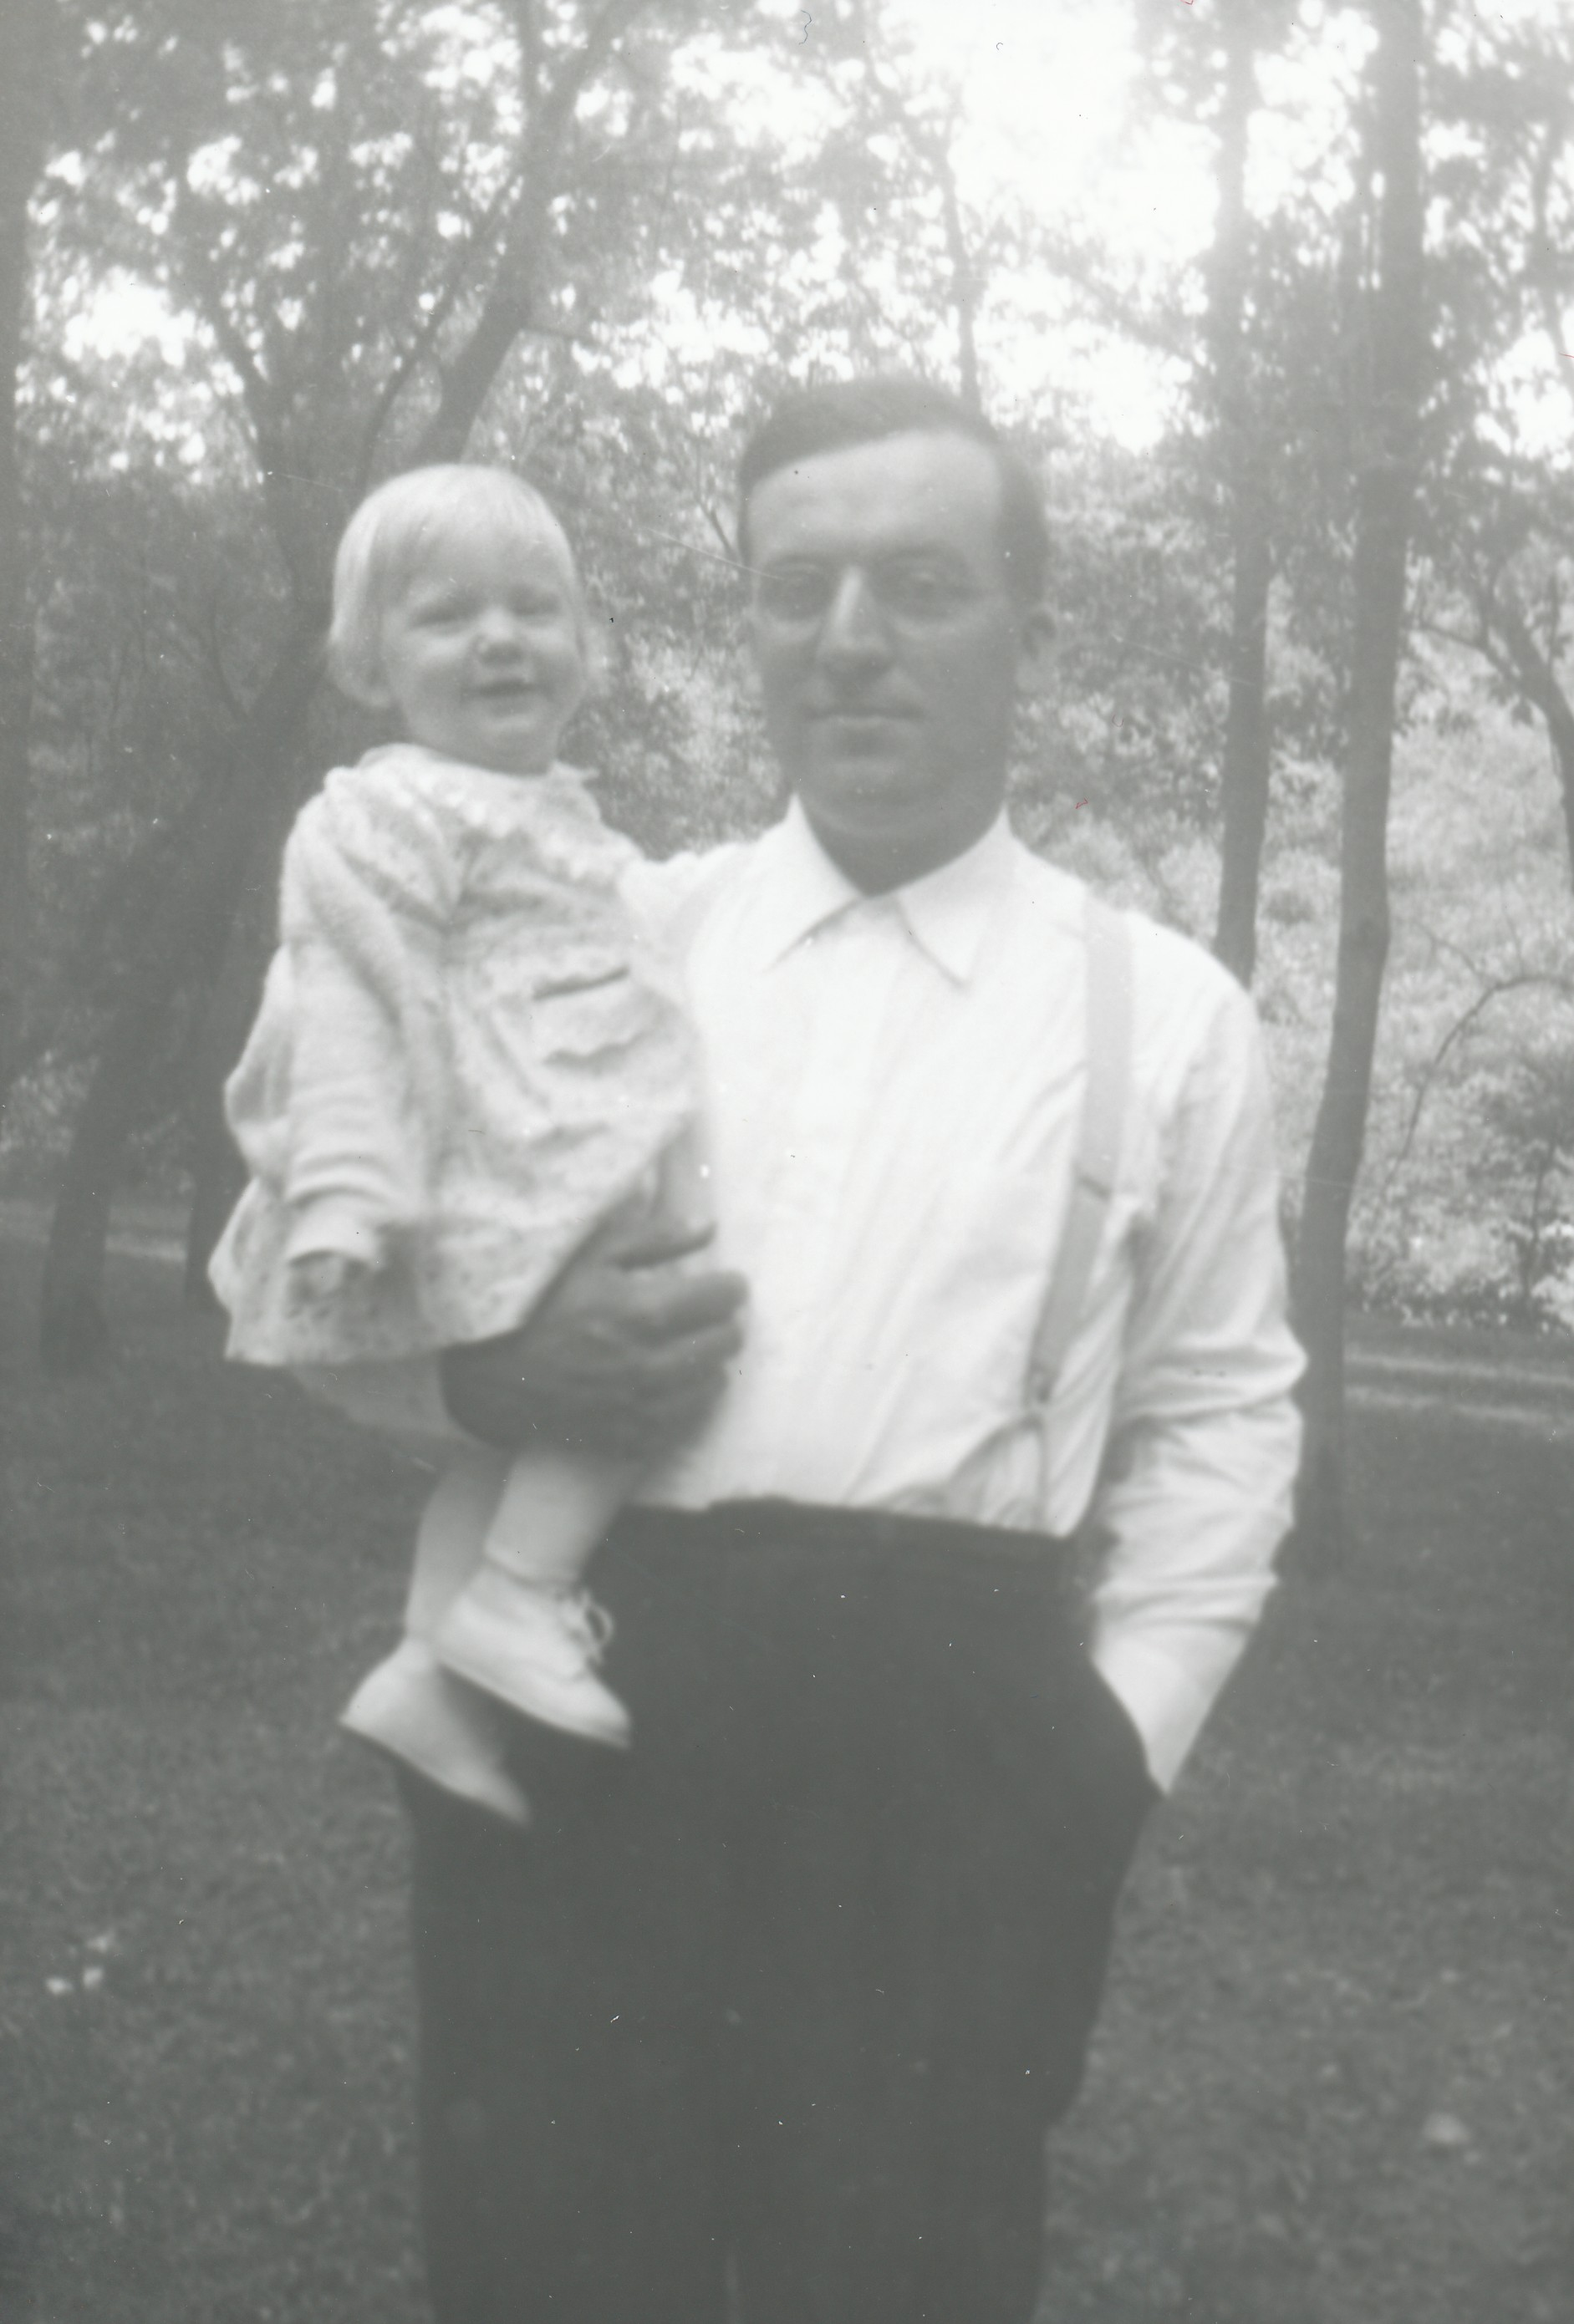
\includegraphics[width=\textwidth]{LoiswithPapa1953}
\caption{Lois with Papa - 1953}
\end{figure}

On summer afternoons it was a relief when he joined the group on the porch to shell peas or lima beans.
The rate of shelling likely doubled when he sat down on the green Adirondack chair and filled his big pan with peas.
The baskets emptied so much faster and the messing around that happened among siblings ceased.
Pop's presence could put an end to misbehavior.
Pop in my book never has to say many words of correction.
It does not take much remembering to bring back the image of Pop with his big hands sitting in the green porch chair or in cold weather in the rocking chair in the corner of the kitchen.
I have an impression memory of sitting on one of his knees across from another sibling on his other knee.
The wallpaper, calendars, linoleum on the floor, the door to the cellar, the kitchen cabinet with one section dedicated to the Bibles and hymnals used for family worship.
Pop could sing and I liked to hear that.
Another impression memory was sitting on his knee during Sunday morning church service.
This meant that I was among the men of the church since the men and women sat on separate sides of the church.

\begin{figure}
\centering
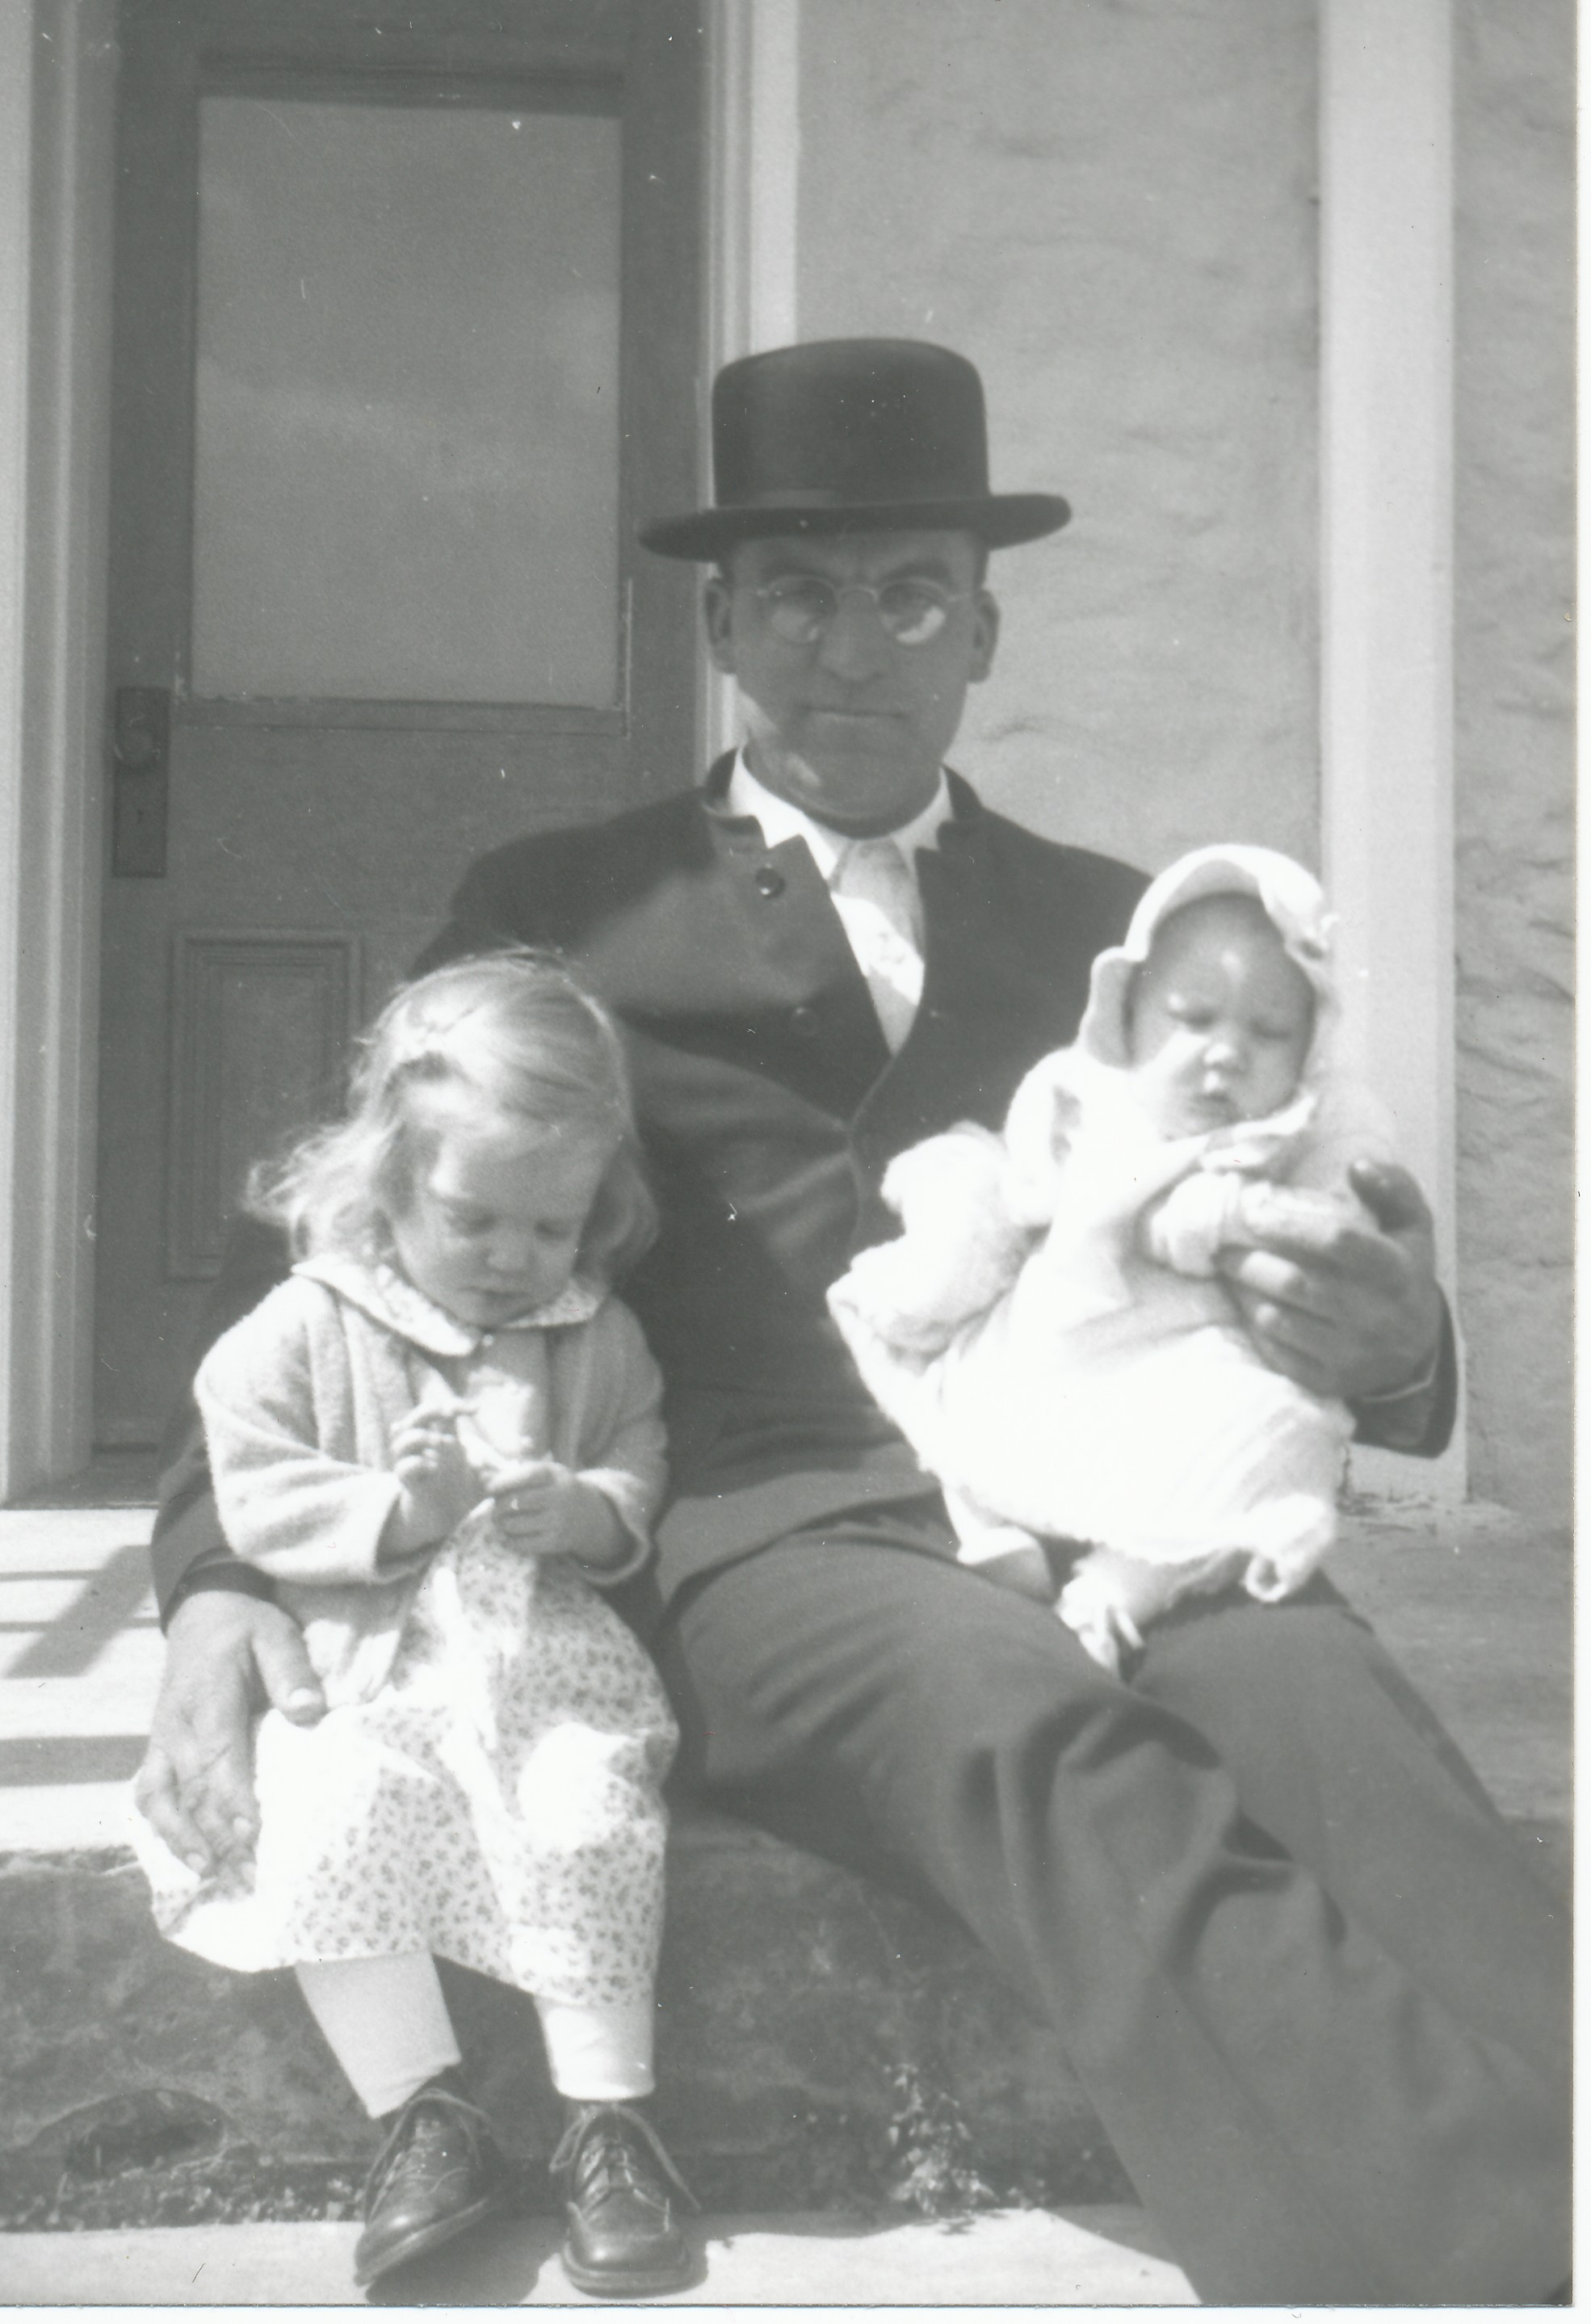
\includegraphics[width=\textwidth]{PapaMaryandLois}
\caption{Papa, Mary, and Lois}
\end{figure}
I liked to see Pop with a twinkle in his eyes and when he laughed he did not laugh out loud but more often silently with his shoulders shaking as he held in his laughter.
One of the ways that he teased Mom was to pull open her apron strings when he walked behind her as she worked at the stove or sink.
It seemed that was one way he made a connection with her among all the clutter of work and children that filled their lives.

Pop had times of significant back aches.
I wonder about that.
I know he worked hard and have memories of seeing his everyday blue work shirt dripping wet with sweat.
He was under a significant amount of pressure to make a success of the farm that he was buying from his mother (my Grandma Hess).
It was troubling to me as a child to know that he was not always well.
I was proud of his ability to hit a homerun during the end of school picnic ball game.
It was during one of those games that he was hit on the neck by a ball leaving his singing voice damaged.

My impression was that he was a big man and while he was 6 feet tall the impression of bigness may have been the perspective of his fourth daughter.
The two picture attached while grainy also convey his impressive presence I felt as a child.

\textbf{Tim's question} - This is quite poignant: "Ironically, given the size of his family it seems he chose to die when he was alone.
My mother had briefly left the room."

Can you remind me of the details of this? Were they still at the house in Millersville? One of my first memories of what has become my classic hard, sustained cry was at a family gathering at the Hess farm after Grandpa's death.
It was one of those moments that have become familiar where I didn't feel a lot of strong emotion and then the grief came on all at once.

I love these photos and they fit so beautifully with this line: "The world seemed a better place when he smiled."

I love this image: "One of the ways that he teased Mom was to pull open her apron strings when he walked behind her as she worked at the stove or sink.
It seemed that was one way he made a connection with her among all the clutter of work and children that filled their lives."

I'm struck strongly by how different my life is from his as I sit here in our quiet living room on a Saturday morning with the dishwasher running in the background.

\textbf{Mom's reply} - "Can you remind me of the details of this.
Were they still at the house in Millersville?" - Tim

They were living in the house in Millersville.
Pop or Grandpa had been getting weaker.
Hospice had been contacted and a hospital bed was going to be moved into the house.
The family in the area had gathered and sang around his bed.
Someone stayed the time with Pop and Mom.
(I'm going from what I remember other family members telling me.) That morning my brother Dave and brother-in-law Rick had both stopped by.
It seemed that Pop did not have long to live.
Rick checked in with him and told Mom that his death was not likely to be immediate.
They both left and Mom was alone with Pop.
She went to the basement to start a load of laundry.
When she came back to his room he was gone.
When I heard that story I thought that seemed congruent with who Pop was.
He was not comfortable being the center of attention and when alone took that time to leave this life and slip away.
It was July 4, 2000.

Grief comes in different ways and at different times.
I remember your weeping and thought it was a good response.
We each respond to grief in our own ways.
I remember experiencing grief for Pop in a cyclic way over the next years.
Something would trigger memories of Pop and there would be a wave of grief.
Grief would recede until there was another trigger perhaps with lessening intensity.


I have feelings about the differences between my life and my parent's lives as well.
Then I think about my life growing up in my family and marvel at the differences between then and now as well.


\textbf{Abby's comment} - This was so lovely Mom.
I am pretty sure I read it closer to when you first wrote it, but I realized I never replied to it.
Your words paint such a wonderful portrait of a man I only knew a small part of.
I am so glad you have such a gift of writing.

